\chapter{Introduzione alla privacy}

Tutto ciò che facciamo online lascia una traccia che è memorizzatile e analizzabile da chi raccoglie i dati personali.

\paragraph{Surveillance Capitalism} Generalmente, tutte le informazione raccolte su di noi vengono date in pasto ad algoritmi di machine learning che le usano per predire il nostro comportamento. In questo modo, i venditori di servizi possono proporci prodotti in linea con i nostri interessi.

\paragraph{Sorveglianza dei governi} Esistono anche altri tipo di surveillance, come quello inglese/americano che raccoglieva dagli IPS i dati sulle comunicazioni internet nei due paesi e le usava per ottenere informazioni sui rispettivi cittadini.

\paragraph{Data breach} Gli enti che raccolgono queste informazioni sono soggetti ad attacchi di data breach. Gli attaccanti, ad esempio, una volta ottenuti i dati di una certa persona potrebbero sfruttarli per effettuare attacchi di phishing spacciandoti per quella persona.

\paragraph{Iniziative a favore della privacy} Negli ultimi anni sono nate diverse iniziative volte a tutelare/garantire la privacy, come il GDPR, Tor, Privacy Badger (previene l'online tracking), Dp3t (protocollo sviluppato da centri di ricerca europei con lo scopo di consentire il tracciamento dei contagi senza rivelare identità degli utenti coinvolti).

\section{Definizione di privacy}
Non è semplice definire la privacy in quanto è un concetto che può avere un significato diverso per ciascun individuo. Nel tempo sono state date delle definizioni più "adottate" di altre:
\begin{itemize}
    \item "Il diritto ad essere lasciato solo";
    \item "Il diritto dell'individuo di decidere quali e quando le proprie informazioni devono essere pubbliche";
    \item "La libertà da vincoli irragionevoli sulla costruzione della propria identità" (se un utente sa che le sue conversazioni sono monitorate, probabilmente limiterà le informazioni scambiate/scriverà in modo diverso);
    \item Tassonomia dei pericoli alla privacy: piuttosto che definire la privacy, definisce tutte quelle attività che portano alla compromissione della privacy;
    \item "Privacy come integrità contestuale": lega la definizione di privacy alla nozione di contesto (in un contesto potrebbe essere appropriato condividere info personale, in altre no.  L’appropriatezza è data da da norme);
    \item Trasparenza, finalità, proporzionalità, responsabilità (dal GDPR):
    \begin{itemize}
        \item Trasparenza: quando un data controller raccoglie i dati, deve specificare quali dati raccoglie e come li tratterà o condividerà.
        \item Purpose: deve specificare il motivo per cui li raccoglie
        \item Proporzionalità: devono essere proporzionali e finalizzati al purpose; non devo raccogliere più dati del necessario
        \item Accountability: il data controller deve mantenere traccia di chi ha accesso ai dati.
    \end{itemize}
\end{itemize}

\section{Proprietà della privacy}
Le proprietà della privacy vengono suddivise in base a due macro definizioni di privacy:
\begin{itemize}
    \item Hard privacy: parte dall'assunzione che il data controller non è un'entità di cui ci si può fidare e quindi l'individuo deve condividere con lui il minor numero di dati sensibili. Sarà l'utente a dover adottare tutte le tecniche per proteggere la propria privacy (es: cifratura);
    \item Soft privacy: l'utente si fida del data controller e quindi è lui a dover adottare tutte le tecniche possibili per minimizzare i rischi per l'utente. Ovviamente in questo caso è più difficile per l'utente avere controllo su come i suoi dati vengono processati o suddivisi dal data controller.
\end{itemize}

\noindent In figura \ref{fig:12-1} sono riportate le proprietà definite per le due definizioni.

\begin{figure}
    \centering
    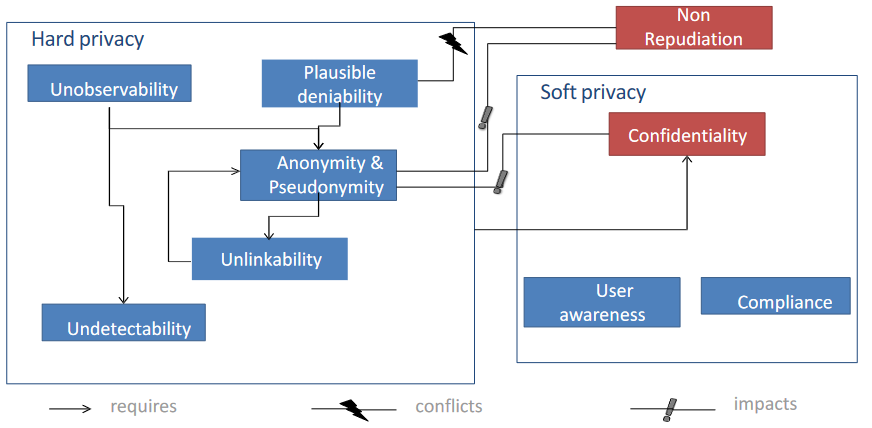
\includegraphics[width=0.8\textwidth]{images/12-1.png}
    \caption{Proprietà delle due definizioni.}
    \label{fig:12-1}
\end{figure}

\noindent Le proprietà sono state definite rispetto ad un preciso modello di attaccante: abbiamo un sistema dove diversi attori compiono azioni e un attaccante monitora le azioni eseguite dagli utenti. In particolare, l'obiettivo dell'attaccante è inferire gli \textbf{item of interest}, informazioni di interesse per l'attaccante (es: contenuto del messaggio, chi è il mettente, chi è il ricevente, ...).

\subsection{Anonimity}
Abbiamo anonimità quando un attaccante non può identificare l'attore all'interno di un gruppo di attori (\textbf{anonimity set}). Praticamente abbiamo anonimità quando, all'interno del sistema, non è possibile legate l'identità di uno degli attori ad un determinato item of interest.

Ad esempio, un attaccante non riesce a determinare quale attore ha spedito o ricevuto un messaggio.

All'interno di una rete, possiamo avere due anonimity set: l'insieme dei possibili mittenti e l'insieme dei possibili riceventi del messaggio. 
\\

\noindent Spesso il concetto di anonimità è legato a quello di \textbf{pseudoanonimità}: invece di usare il vero nome per identificare un soggetto si usa un ID casuale. Questo comporta che, se un utente usa sempre lo stesso ID, siamo in grado di tracciare tutte le azioni che ha effettuato.

\subsection{Unlinkability}
Nasconde la presenza di un collegamento tra due item of interest. Se la proprietà è soddisfatta, un attaccante non deve essere, ad esempio, in grado di determinare se due messaggi appartengono alla stessa sessione, oppure se sono stati mandati dallo stesso utente.

L'unlinkability può essere usata anche per definire l'anonimity. Quest'ultima non  altro che un'unlinkability tra due item of interest: l'identità dell'utente e le azioni che questo ha compiuto all'interno del sistema

\subsection{Undetectability}
Sotto questa proprietà cadono due sotto-proprietà:
\begin{itemize}
    \item Undetectability: se un attaccante osserva la rete non è in grado di determinare se un dato item of interest esiste oppure no. Supponiamo che il nostro item of interest sia un messaggio, l'attaccante non deve essere in grado di distinguere tra messaggio inviato e rumore casuale sulla rete;
    \item Unobservability: assume che l'undetectability valga per tutti gli utenti della rete non coinvolti nello scambio del messaggio. Inoltre vuole l'anonimità di ciascun soggetto coinvolto nell'item of interest rispetto agli altri (il mettente non sa chi sarà il ricevente e il ricevente non sa chi è il mittente del messaggio -> in un database medico non possiamo dire se un record esiste; non possiamo dire se una persona ha visitato un dato sito web);
\end{itemize}

\subsection{Plausible deniability}
Va in contrasto con la non repudiation. Garantisce che un utente possa negare di aver visitato una data pagina web, aver spedito una data email o aver detto qualcosa. 

Questa proprietà può essere desiderabile, ad esempio, nei sistemi di online voting. Al contrario, in siti di e-commerce, è desiderabile il contrario, quindi la non-repudiation.

\subsection{Confidentiality}
Prevede che sia responsabilità del data controller proteggere i dati da un accesso non autorizzato. In pratica si traduce nella cifratura dei dati o nell'utilizzo di meccanismi di controllo dell'accesso.

\subsection{Compliance}
É legata al rispettare i principi dettati dalle leggi sulla protezione dei dati personale, come i principi dettati dal GDPR.

\subsection{Awareness}
Più legata all'utente che al data controller, prevede che l'utente sia messo a conoscenza della conseguenza del condividere informazioni (es: l'utente posta la foto della carta di credito online senza nascondere i codici). Si focalizza sul garantire che, quando l'utente condivide i propri dati personali, lo faccia in maniera coscienziosa. 

\section{Minacce alla privacy}
Solove si è focalizzato su come la privacy possa essere compromessa. Dalla sua analisi, è riuscito a definire quattro categorie di azioni che possono compromettere la privacy. Tre di queste sono mappate sulle azioni che un data controller esegue quando raccoglie dati su un individuo:
\begin{enumerate}
    \item Information collection, che consiste nella raccolta di dati dell'utente;
    \item Information processing, che consiste nell'elaborazione dei dati raccolti;
    \item Information dissemination, che consiste nella condivisione dei dati elaborati con parti terze;
    \item Invasion: non legata generalmente al data controller, racchiude tutte quelle situazioni in cui la sfera privata dell'individuo viene compromessa.
\end{enumerate}

\subsection{Information collection}
Comprende due tipi di attacchi:
\begin{itemize}
    \item Surveillance: le attività che un individuo compie vengono osservate e registrate. Alcuni esempi possono essere:
    \begin{itemize}
        \item Contatori smart: danno informazioni più precise, riducendo quindi i costi, ma allo stesso tempo permettono di inferire info sull'utente, come quante docce si fa.
        \item Angry birds era usata dalla NSA per raccogliere info.
    \end{itemize}
    \item Interrogation: le informazioni sono estorte dall'individuo (lo si convince a fornire informazioni che normalmente non fornirebbe). Esempi possono essere:
    \begin{itemize}
        \item Probing: attacchi di phishing che richiedono agli utenti di resettare login e password.
    \end{itemize}
\end{itemize}


\subsection{Information processing}
Comprende cinque tipi di attacchi:
\begin{enumerate}
    \item \textbf{Aggregation}: il data controller raggruppa le informazioni su un individuo da diverse sorgenti, e impara nuove informazioni che l’individuo non pensava sarebbero state inferite. Esempi:
    \begin{itemize}
        \item Target ha predetto che una cliente era incinta (prima che lei lo sapesse) tramite le transazioni catturate dalla "carta fedeltà" e ha iniziato a inviare coupon su prodotti per la maternità.
    \end{itemize}
    \item \textbf{Identification}: il data controller raggruppa una serie di informazioni e riesce a trovare l’identità del soggetto.
    \begin{itemize}
        \item Un'azienda americana è riuscita a raccogliere i dati sui click di un individuo su vari siti e dall'analisi di questi dati è riuscita a determinare nome e cognome dell'utente.
    \end{itemize}
    \item \textbf{Insecurity}: il data controller non adotta le misure di sicurezza necessarie per prevenire un accesso non autorizzato.
    \item \textbf{Secondary use}: il DC raccoglie i dati per uno scopo e poi li riutilizza per qualcos'altro senza informare il soggetto. Esempi;
    \begin{itemize}
        \item Un medico raccoglie dati sul paziente li fornisce ad una casa farmaceutica;
        \item Cambridge analytica: genera profili psicologici sugli utenti di facebook poi usati per influenzare la campagna elettorale in America.
    \end{itemize}
    \item Esclusione: l’utente non ha visione di quali sono i dati raccolti dal data controller (non c'è trasparenza).
\end{enumerate}

\subsection{Information dissemination}
Comprende sette possibili attacchi:
\begin{enumerate}
    \item \textbf{Breach of confidentiality}: si verifica un accesso non autorizzato ai dati mantenuti dal data controller. Esempi:
    \begin{itemize}
        \item Equifax: società di recupero crediti che analizzava il credit store (valuta la capacità di un individuo a pagare un debito) dei cittadini americani e inglesi. Questi dati sono state rese pubbliche.
    \end{itemize}
    \item \textbf{Disclosure}: info su una data persona vengono divulgate. Queste info possono influenzare le opinioni delle persone su quell'individuo. Esempi:
    \begin{itemize}
        \item  Icloud nel 2014 leakka immagini di attrici americane in situazioni intime. Le vittime avevano ricevuto una mail di phishing in cui si chiedeva di resettare la password di iCloud.
    \end{itemize}
    \item \textbf{Exposure}: vengono rese pubbliche nudità o dolori di una persona;
    \item \textbf{Increased accessibility}: si aumenta l'audience con la quale si condividono le informazioni;
    \item \textbf{Blackmail}: si minaccia di diffondere dati personali di un individuo se non viene pagato un riscatto. Esempi:
    \begin{itemize}
        \item Ransomware;
    \end{itemize}
    \item \textbf{Appropriation}: i dati personali di una persona vengono usati per impersonarla. Esempi:
    \begin{itemize}
        \item Reti sociali (es: facebook): molte info personali vengono condivise e possono essere usate per impersonarci verso servizi online.
    \end{itemize}
    \item \textbf{Distortion}: si diffondono info false per cambiarne l'opinione degli altri su qeulla persona. Esempi:
    \begin{itemize}
        \item Troll;
    \end{itemize}
\end{enumerate}

\subsection{Invasion}
Comprende tre attacchi:
\begin{enumerate}
    \item \textbf{Intrusion}: situazioni dove altri individui o governi interferiscono con la vita privata di una persona.  Esempi:
    \begin{itemize}
        \item Reti sociali e stalking: femminicidi nonostante gli ordini restrittivi. Il colpevole stalkera la vittima tramite i social;
        \item Cyberbullismo.
    \end{itemize}
    \item \textbf{Decisional interference}: comporta l'incursione del governo nelle decisioni dell'interessato riguardanti il suo privato.
\end{enumerate}

\section{Privacy Enhancing Technologies (PETS)}
Con Privacy Enhancing Technologies intendiamo tutti quei tool, tecnologie e software che ci permettono di proteggere la privacy di un individuo, minimizzandone i rischi. Queste tecnologie possono essere applicate sia dal data subject (utente) oppure dalle organizzazione che raccolgono/analizzano i dati. Possono essere applicate a diversi livelli: rete, browser, database. 

Esistono diverse categorie di tecnologie.

\subsection{Data Protection technologies}
Hanno lo scopo di garantire la proprietà di compliance con i principi di protezione dei data stabiliti dal GDPR. Tipicamente sono adottate dal data controller. Alcuni esempi possono essere:
\begin{itemize}
    \item Cifratura dei dati, sia durante la trasmissione che durante la memorizzazione;
    \item Controllo dell'accesso in base allo scopo per cui i dati sono stati raccolti (si può accedere al dato solo se lo scopo è in linea al motivo per cui sono stati raccolti);
    \item Sistemi di log, per garantire l'accountability;
    \item Fornire un'interfaccia all'utente che permette di cancellare i dati;
    \item Autenticazione e autorizzazione dei lavoratori che accedono ai data.
\end{itemize}

\noindent Si assume che il data controller sia fidato, mentre non ci si fida di tutti le entità esterne che potrebbero accedere ai dati. Non c'è garanzia che il data controller usi i dati per scopi diversi da quelli per cui sono stati raccolti.

\subsection{User awareness technologies}
Insieme di tecnologie il cui scopo è dare all'utente il controllo su quali dati personali vengono raccolti e come vengono usati dal data controller oppure aiutare l'utente a configurare la propria privacy in modo da minimizzare attacchi che possano portare alla divulgazione dei dati personali. Alcuni esempi possono essere:

\begin{itemize}
    \item Privacy settings by defaults: quanto creiamo un account, se chi ha sviluppato il sito ha rispettato i principi di privacy by design e privacy by default, dovrebbe adottare delle impostazioni che proteggano i dati in automatico;
    \item Tool per capire con chi stiamo condividendo le informazioni: facebook permetteva di vedere quello che gli altri vedevano del nostro profilo;
    \item Privacy policy comprensibili: sistemi a layer che permettono di andare ad approfondire ogni aspetto della politica;
    \item Privacy nudges: permettono di vedere quante volte una info personale è stata condivisa e con chi.
\end{itemize}

\subsection{Anonimity technologies}
Hanno l'obiettivo di soddisfare l'anonimità. Alcuni esempi possono essere:
\begin{itemize}
    \item K-Anonimity, per i database;
    \item Sistemi di comunicazione anonima, come Tor;
    \item Sistemi che garantiscono l'anonimità durante l'autenticazione: per garentire la privacy anche nei confronti dell'Identity Provider, che ha visioni su tutti gli Identity Attributes, è stato ideato il sistema di autenticazione Idemix, basato sulla zero-knowledge.
\end{itemize}

\subsection{Altre tecnologie}

\begin{itemize}
    \item Memorizzazione sicura sul cloud: PrivateStorage fornisce una cifratura lato client. I dati sono cifrati prima di uploadare e la chiave simmetrica è conosciuta solo dal client;
    \item Searchable encryption: consente di ricercare se un documenti cifrato contiene determinate parole chiave e di recuperare questi documenti che poi vengono decifrate dal client. Si usa quando l'utente cifra i dati prima di uploadarli. Si evita di dover scaricare tutti i dati, decifrarli e ricercare il documento che serve;
    \item Computazioni su dati cifrati: Homomorfic encryption (poco usata in quanto poco efficiente) o Secure multiparty computation (un insieme di utenti che vogliono calcolare una determinata funzione sulla base di input di ciascun utente, ma vogliono anche mantenere privati gli input).
\end{itemize}








